In this chapter, we present our reference CPU application.
We also present an experimental setup, which we use the performance of the FM-index implementations.

\section{Reference implementation} \label{section:reference_cpu}

To analyze the performance of an FPGA implementation, we have programmed a CPU-based reference implementation in the C language.
We have chosen this language for its performance and for easy portability to an FPGA kernel written in C, C++ or OpenCL.
As will be explained in section \ref{section:experiment_setup}, we will focus on analyzing the performance of string-matching, and not the construction of the FM-index.
Therefore we can precalculate all auxiliary data structures that were previously explained in section \ref{section:background_stringmatching}.

\subsection{Interface} \label{section:cpu_interface}

The data structures comprising the FM-index are implemented as a C struct shown in listing \ref{listing:fmindex_struct}.
The suffix array is henceforth abbreviated as \cinline{sa} in code listings.

\begin{listing}[H]
\begin{minted}{c}
typedef unsigned ranges_t;
typedef unsigned ranks_t;
typedef unsigned sa_t;

typedef struct fm_index {
  char *bwt;
  size_t bwt_sz;
  char *alphabet;
  size_t alphabet_sz;
  ranks_t *ranks;
  sa_t *sa;
  ranges_t *ranges;
} fm_index;
\end{minted}
\caption{The C struct for the FM-index. The \cinline{bwt}, \cinline{ranks} and \cinline{sa} data structures correspond to the Burrows-Wheeler transform, rank matrix and suffix array respectively. The data structure \cinline{ranges} is used to lookup a character in the Burrows-Wheeler matrix.}
\label{listing:fmindex_struct}
\end{listing}

The exposed functions are presented in listing \ref{listing:fmindex_functions}.
The \cinline{FMIndexConstruct} function constructs the FM-index from the given text, and \cinline{FMIndexFree} frees the FM-index and all underlying data structures.
The functions \cinline{FMIndexDumpToFile} and \cinline{FMIndexReadFromFile} can be used to save and read an FM-index to and from a file. 
The flag \cinline{aligned} specifies whether to allocate memory page-aligned, which is useful for communication with the FPGA in chapter \ref{chapter:fpga}.
Finally, the \cinline{FMIndexFindMatchRange} and \cinline{FMIndexFindRangeIndices} functions are used to find the indices of a given pattern within a text, as explained in section \ref{section:background_fmindex}.
\cinline{FMIndexFindMatchRange} finds the start and end of the range of matches for a pattern, and saves these in \cinline{start} and \cinline{end} respectively.
\cinline{FMIndexFindRangeIndices} finds all indices using the earlier acquired range, and saves them in \cinline{match_indices}.

\begin{listing}[H]
\begin{minted}{c}
fm_index *FMIndexConstruct(char *s);
void FMIndexFree(fm_index *fm);

int FMIndexDumpToFile(fm_index *fm, char *filename);
fm_index *FMIndexReadFromFile(char *filename, int aligned);

void FMIndexFindMatchRange(fm_index *fm, char *pattern, size_t pattern_sz,
                           ranges_t *start, ranges_t *end);
void FMIndexFindRangeIndices(fm_index *fm, ranges_t start, ranges_t end,
                             unsigned long **match_indices);
\end{minted}
\caption{The FM-index C functions exposed by the interface.}
\label{listing:fmindex_functions}
\end{listing}

\subsection{String searching} \label{section:string_searching}

The two functions from section \ref{section:cpu_interface} to perform string searching using the FM-index are shown in full in listing \ref{listing:string_searching}.
The \cinline{FMIndexFindMatchRange} function closely follows the pseudocode in listing \ref{listing:bw_occurences}.
The \cinline{FMIndexFindRangeIndices} uses the found range of matches, and performs a simple lookup in the suffix array to find the original indices.

\begin{listing}[H]
\begin{minted}{c}
void FMIndexFindMatchRange(fm_index *fm, char *pattern, size_t pattern_sz,
                           ranges_t *start, ranges_t *end) {
  int p_idx = pattern_sz - 1;
  char c = pattern[p_idx];

  *start = fm->ranges[2 * string_index(fm->alphabet, c)];
  *end = fm->ranges[2 * string_index(fm->alphabet, c) + 1];

  p_idx -= 1;
  while (p_idx >= 0 && *end > 1) {
    c = pattern[p_idx];
    ranges_t range_start = fm->ranges[2 * string_index(fm->alphabet, c)];
    int alphabet_idx = string_index(fm->alphabet, c);
    *start =
        range_start + fm->ranks[fm->alphabet_sz * (*start - 1) + alphabet_idx];
    *end = range_start + fm->ranks[fm->alphabet_sz * (*end - 1) + alphabet_idx];
    p_idx -= 1;
  }
}

void FMIndexFindRangeIndices(fm_index *fm, ranges_t start, ranges_t end,
                             unsigned long **match_indices) {
  for (unsigned long i = 0; i < end - start; ++i)
    (*match_indices)[i] = fm->sa[start + i];
}
\end{minted}
\caption{The full implementation of string searching using the FM-index.}
\label{listing:string_searching}
\end{listing}

\subsection{Burrows-Wheeler transform construction} \label{section:bwt_construction}

We previously explained in section \ref{section:background_bwt} that, in order to obtain $\Tbw$, we list all rotations of the text and then lexicographically sort them.
This would unfortunately lead to a space complexity of $O(n^2)$ which is infeasible for large data sets.
To avoid this issue, we can derive $\Tbw$ from the suffix array of the text \cite{ullah_implementation_2020}.
The suffix array is essentially a Burrows-Wheeler transform, but holds indices instead of characters.
Deriving $\Tbw$ is therefore as easy as indexing the text for each index in the suffix array.

The C code for obtaining the suffix array from a text is shown in listing \ref{listing:construct_sa}.
First we simply list all indices of the text.
Then we use quicksort to sort the indices: for each pair of indices, the strings starting from these positions are lexicographically compared.

\begin{listing}[H]
\begin{minted}{c}
sa_t *ConstructSuffixArray(char *text, size_t text_sz) {
  sa_t *suffix_array = calloc(text_sz + 1, sizeof(sa_t));

  for (size_t i = 0; i < text_sz + 1; ++i)
    suffix_array[i] = i;

  qsort_r(suffix_array, text_sz + 1, sizeof(sa_t), &CompareSuffixArray, text);

  return suffix_array;
}
\end{minted}
\caption{Generating the suffix array for a text. The auxiliary function \texttt{CompareSuffixArray} lexicographically compares two suffixes, taking the sentinel character \texttt{\$} into account which is always sorted first.}
\label{listing:construct_sa}
\end{listing}

\section{Experimental setup \& hypothesis} \label{section:experiment_setup_hypo}

\subsection{Experimental setup} \label{section:experiment_setup}

We investigate the performance on the CPU and FPGA using two metrics found in literature.
To evaluate the overall performance, throughput is measured by counting the average amount of patterns matched (finding the corresponding original positions) per second.
Additionally, to provide a more fair comparison between CPU and FPGA, the throughput is also expressed as the amount of patterns matched per clock cycle.
As one of the main benefits of FPGAs is energy efficiency, we also evaluate average energy usage for matching one pattern.

The string searches are performed on FM-indices which we preprocess on the CPU.
We use several corpora provided by the Pizza \& Chili corpus collection \cite{ferragina_pizzachili_nodate} to compute the FM-indices.
This collection is often used for text compression and indexing, and features corpora from a diverse set of sources \cite{makinen_compressed_2007}.
We use the \textit{dna}, \textit{proteins} and \textit{dblp.xml} corpora for our experiments.
An explanation for each corpus and the alphabet size is shown in table \ref{table:corpora}.

\begin{table}[H]
  \begin{tabularx}{\linewidth}{l X l}
    \hline
    \textbf{Corpus} & \textbf{Description} & \textbf{$|\Sigma|$} \\ \hline
    \textit{dna} & DNA sequences provided by Project Gutenberg. The DNA bases are encoded as A, C, G and T, but also contains special characters. & 16 \\ \hline
    \textit{proteins} & Protein sequences provided by the Swiss-Prot database. The 20 amino acids are encoded as upper-case letters. Also contains special characters. & 27 \\ \hline
    \textit{dblp.xml} & Bibliographic information on computer science journals in XML format, provided by DBLP. & 97 \\ \hline
  \end{tabularx}
  \caption{Description and alphabet size of the three corpora used from the Pizza \& Chili corpus collection.}
  \label{table:corpora}
\end{table}

To measure throughput, we generate as input for the experiment 7500 random patterns that occur in the text.
Generating random patterns from the alphabet alone gives too many patterns that have no occurences in the original text, especially for the \textit{dblp.xml} corpus which has a high alphabet size.
We therefore think taking patterns that actually occur in the original text better reflects a normal string search.
We experiment with different pattern lengths, namely lengths 4, 6 and 8.
We chose these lengths because smaller lengths would give way too many matches for corpora with a small alphabet size, while bigger lengths would give almost no matches at all for a large alphabet size.

We also investigate the effect of the size of the corpus on the throughput.
Therefore, for each corpus, we perform experiments on 10, 15 and 20 MB versions of the corpus.

Lastly, each experiment is performed five times to limit variability.

The CPU experiments are performed on an Intel Xeon Gold 6128 processor \cite{noauthor_intel_nodate}.
This CPU has a base frequency of 3.40 GHz.

\subsection{Hypothesis} \label{section:cpu_hypothesis}

We expect that a higher pattern length will result in a lower throughput, as string searching using the FM-index loops over the characters of the pattern.
Subsequently, we expect that the size of the corpus has a negligible effect on the throughput.
Lastly, we hypothesize that corpora with a larger alphabet, i.e. the \textit{dblp.xml} corpus, have a lower throughput, as the data structures are larger which could negatively impact memory performance.


\section{Results} \label{section:results_cpu}

Figure \ref{fig:throughput_cpu} shows the average throughput of the three corpora with different pattern length and corpus sizes.
The top throughputs reach more than 400 thousand patterns matches per second, while we also see some in the lower ten thousands.

We see that, contrary to the hypothesis, a longer pattern generally leads to higher throughput.
To explain this fact, we plot how many occurences a pattern has in the original text on average in figure \ref{fig:match_count_cpu}.
Not surprisingly we see that longer patterns have less occurences than shorter ones.
For shorter patterns, we therefore have to look up way more positions in the suffix array.
The memory lookups explain why longer patterns in figure \ref{fig:throughput_cpu} are faster to search for.

When we look at the effect of the corpus size, we see that for the \textit{dna} and \textit{dblp.xml} corpora, a bigger text leads to lower throughputs.
However, the lower throughput does not seem to be linear to the corpus size.
We think the lower throughput could be the result of memory caching, as random accesses in the data FM-index data structures are more likely to result in page faults.

\begin{figure}[H]
\centering
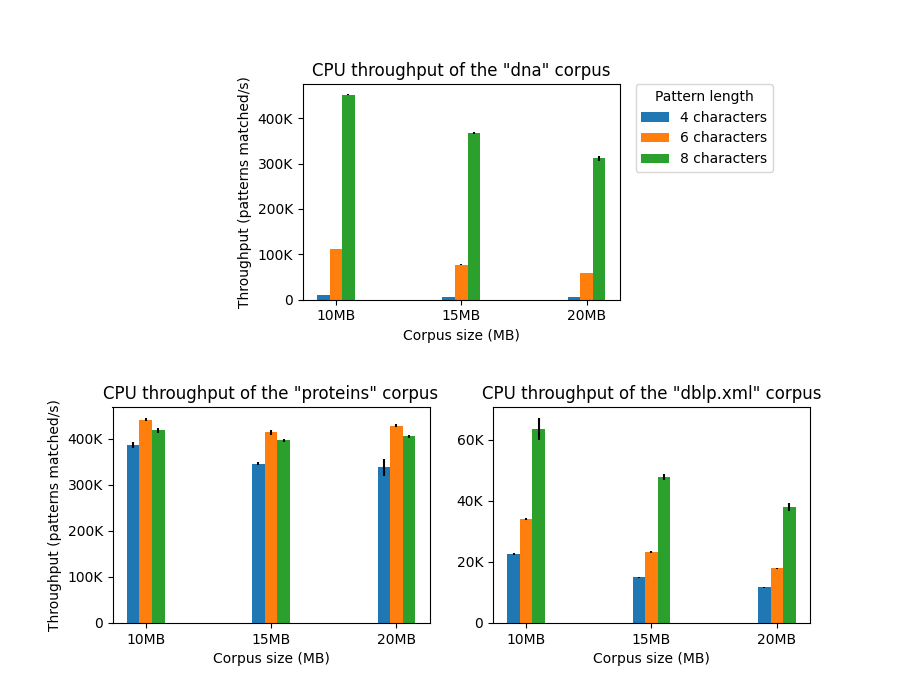
\includegraphics[width=1.0\textwidth]{figures/throughput_cpu.png}
\caption{Average throughput over 5 runs for the CPU reference application. The \textit{dna}, \textit{proteins} and \textit{dblp.xml} corpora are showns for different pattern lengths and corpus sizes. Note that the y-axis has a different scale for each figure.}
\label{fig:throughput_cpu}
\end{figure}

We also observe that the \textit{proteins} corpus has a comparable throughput independent of corpus size or pattern length.
If we again look at figure \ref{fig:match_count_cpu}, we see that more all pattern lengths the average amount of occurences of a pattern is very low compared to the other corpora.
This is seemingly a property of this corpus: the text is apparantly very random and any pattern does not occur very often.

Lastly, we do indeed see that the \textit{dblp.xml} corpus with the high alpabhet size has a throughput almost 7x lower than the other two corpora.
Whether this is the result of worse caching, is not known.

\begin{figure}[H]
\centering
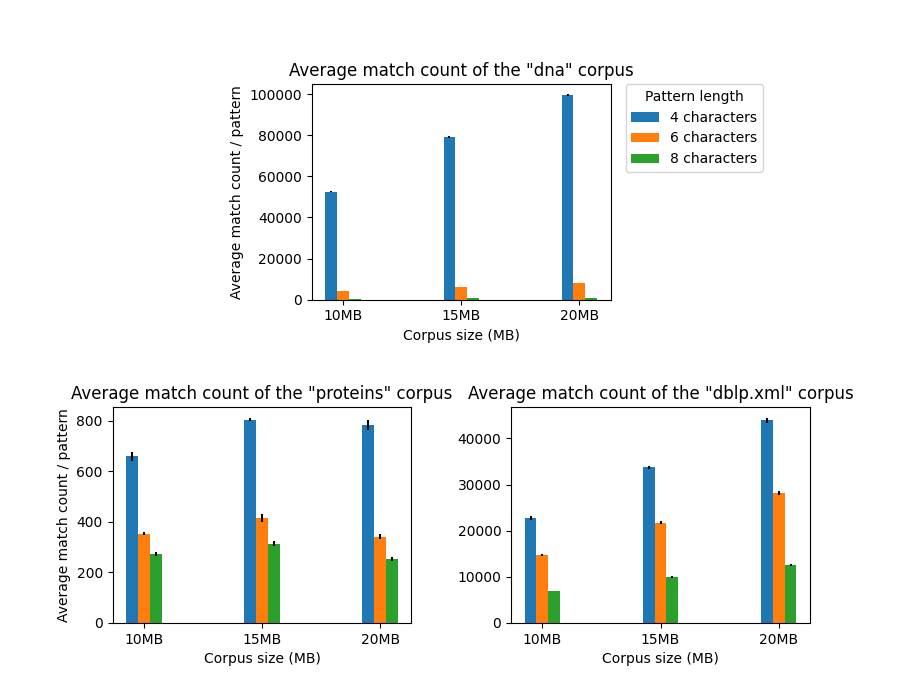
\includegraphics[width=1.0\textwidth]{figures/match_count_cpu.png}
\caption{Average amount of matches per pattern over 5 runs for the \textit{dna}, \textit{proteins} and \textit{dblp.xml} corpora for different pattern lengths and corpus sizes. Note that the y-axis has a different scale for each figure.}
\label{fig:match_count_cpu}
\end{figure}
